\chapter{CMOS Inverter}
\begin{figure}[h]
  \centering
  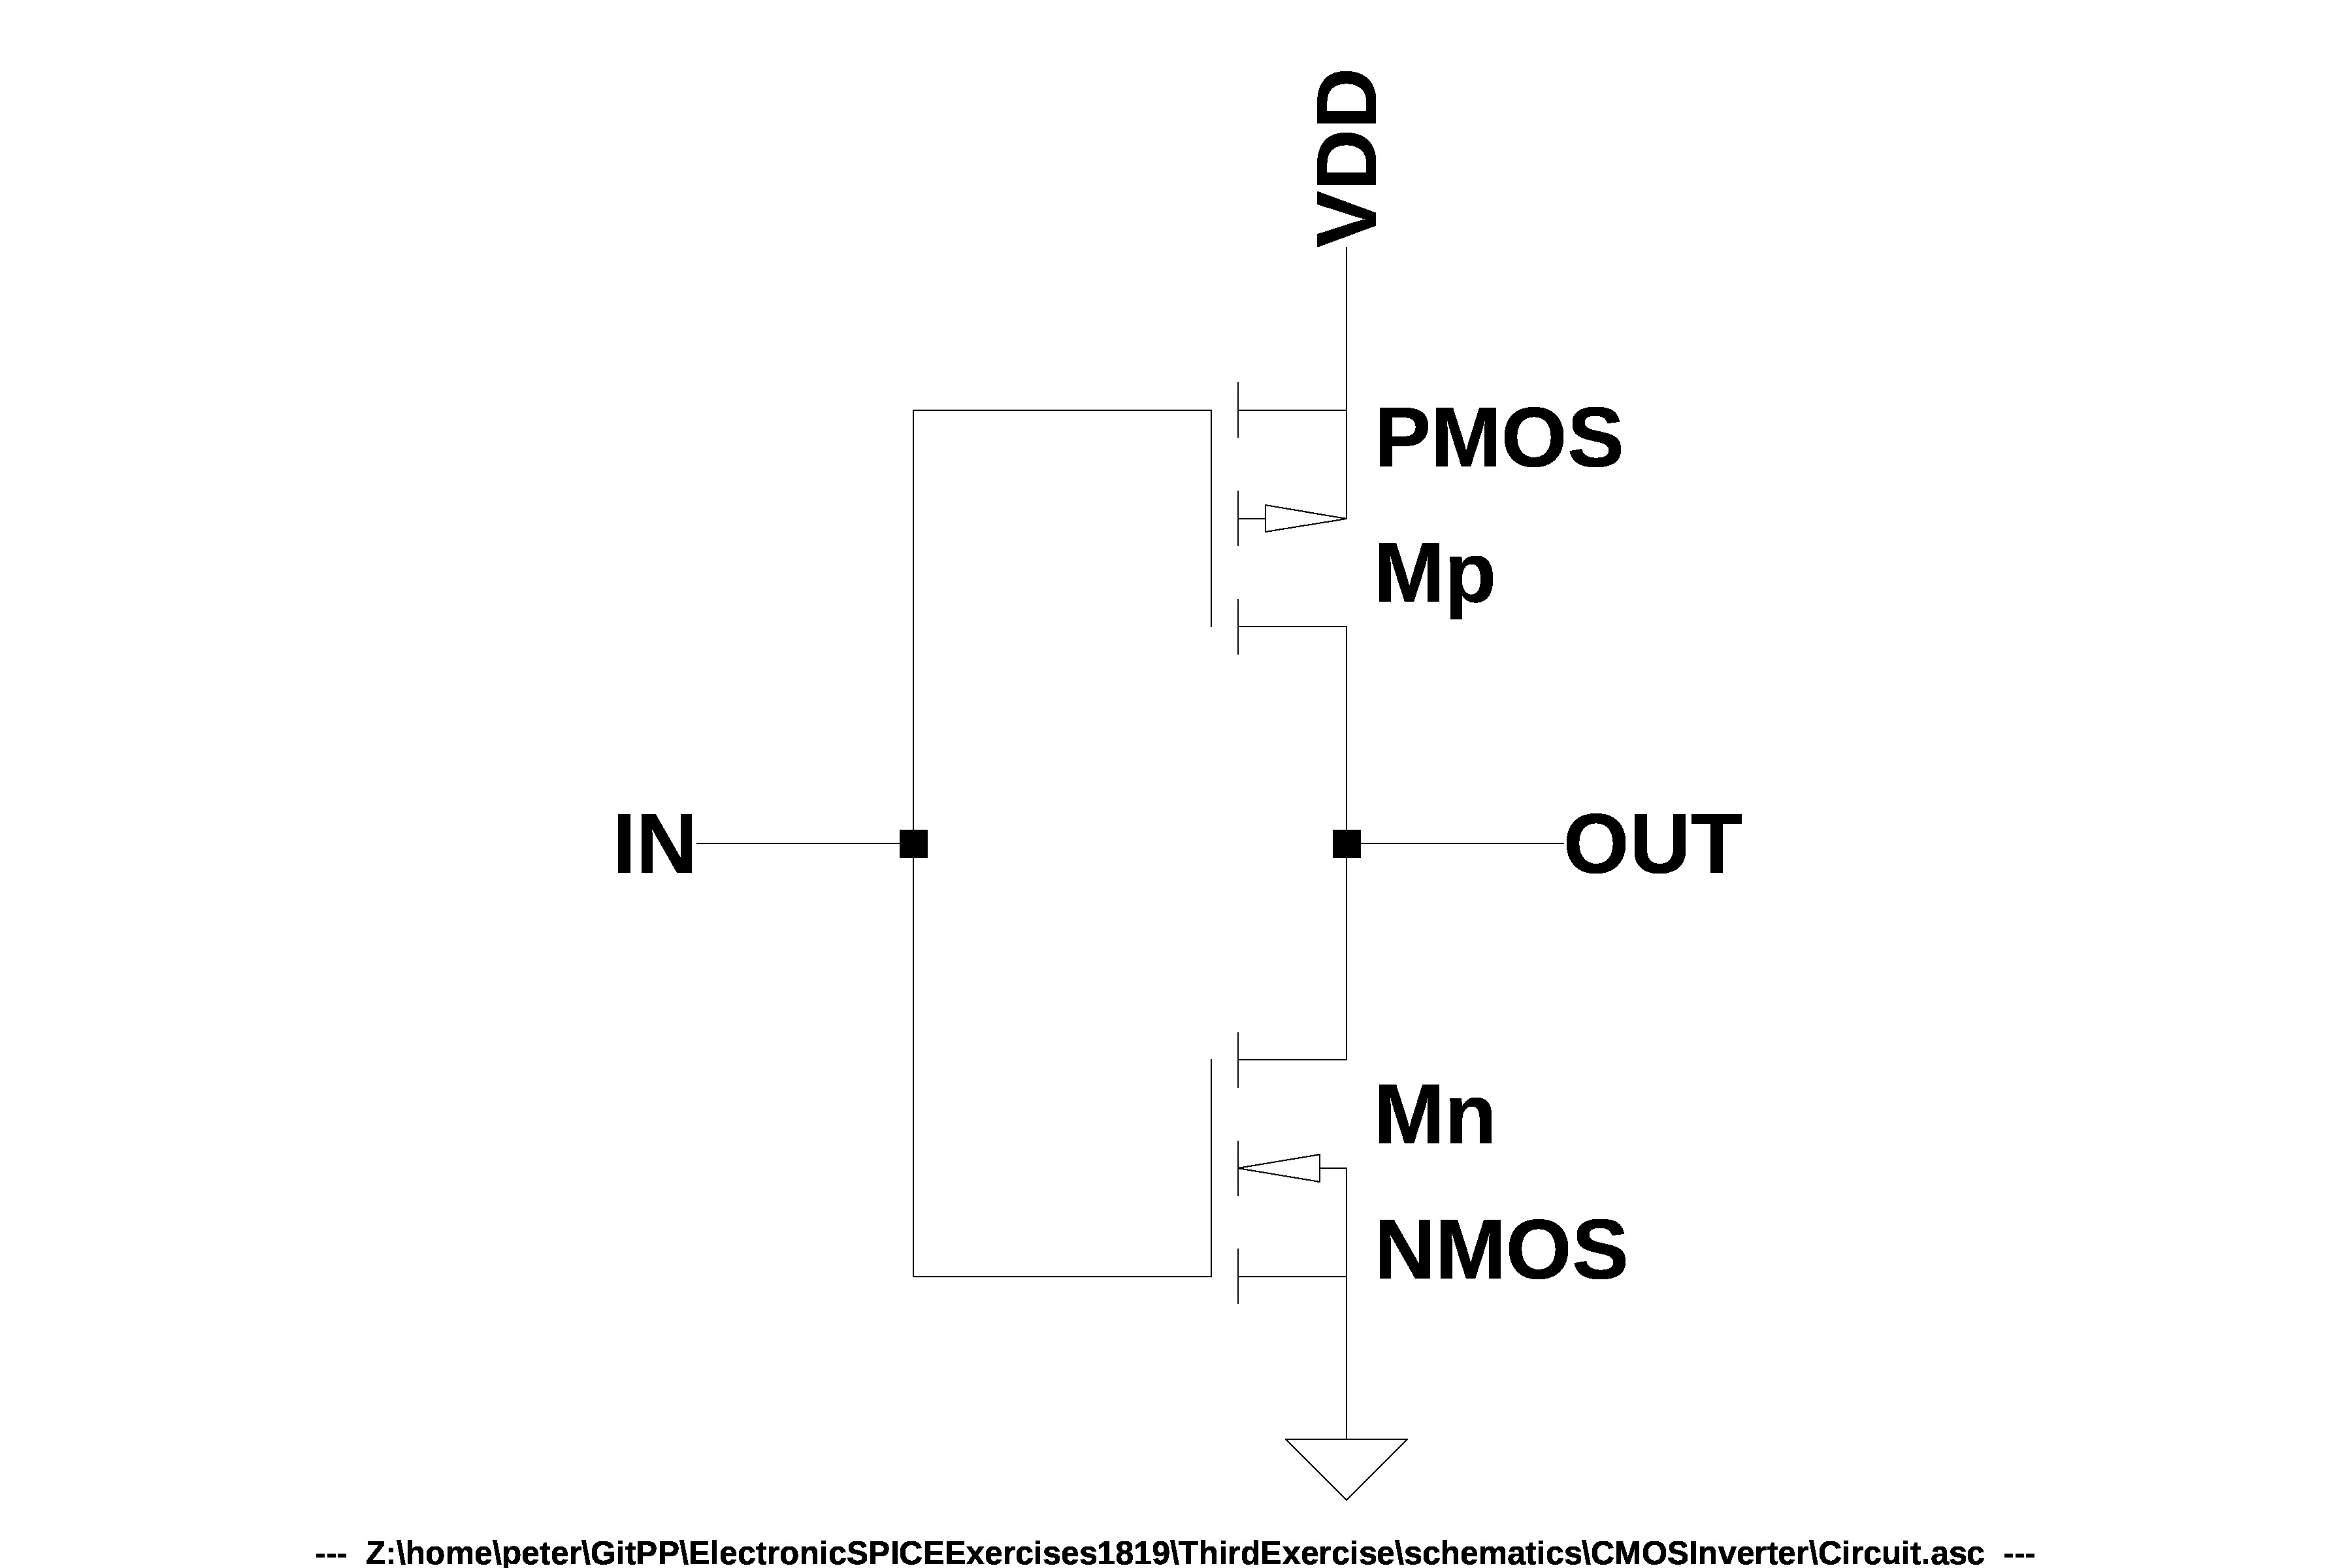
\includegraphics[width=12cm]{schematics/CMOSInverter/Circuit.jpg}
  \caption{CMOS Inverter}
  \label{CMOSInverterCircuit}
\end{figure}
  
\section{Initial data} \label{CIInitialData}
\begin{align}
V_{DD} = 5V
\end{align}

\begin{align} \label{mn}
M_n \left\{
\begin{array}{l}
V_t = 0.7V\\
K'_n = \mu _n C_{ox} = 48 \mu A / V^2\\
\lambda = 0.01 V^{-1}
\end{array}
\right.
\end{align}

\begin{align} \label{mp}
M_p \left\{
\begin{array}{l}
V_t = 0.7V\\
K'_p = \mu _p C_{ox} = 12 \mu A / V^2\\
\lambda = 0.01 V^{-1}
\end{array}
\right.
\end{align}

\section{Dimensioning a balanced inverter}
The conditions for a balanced inverter is on equation \ref{balanced}.\\
It's granted that the transfer function of the inverter is symmetrical.\par
\begin{align}
\frac{W_p}{W_n} = \frac{\mu _p}{\mu _n} \label{balanced}
\end{align}

The length of the channel is usually setted to the minimum length of the fabrication process.\\
In this case it's supposed to be as in the equation \ref{ChannelLength}.\par
\begin{align}
L_p = L_n = 50 nm \label{ChannelLength}
\end{align}

Furthermore, in order to minimizing the area of the integrated circuit, the weight-length's rapport of the NMOS is usually setted between $1$ and $1.5$.\\
In this case it's supposed to be as in the equation \ref{wlrapport}. \par
\begin{align}
\frac{W_n}{L_n} = 1 \label{wlrapport}
\end{align}

So in the equations \ref{wn} and \ref{wp} there is the weight of the MOSFET's circuit.\\

\begin{align}
\frac{W_n}{L_n} = 1 \implies W_n = L_n \xRightarrow{(eq. \ref{ChannelLength})} W_n = 50nm \label{wn}
\end{align} 

\begin{align}
\frac{W_p}{W_n} = \frac{\mu _p}{\mu _n} \implies W_p = \frac{\mu _p}{\mu _n}W_n \xRightarrow{(eq. \ref{mn}, \ref{mp}, \ref{wn})} W_p = \frac{48 \mu A / V^2}{12 \mu A / V^2} \cdot 50nm = 200nm
\end{align}

\subsection{Resuming}
\begin{center}
\begin{tabular}{|c|c|c|c|c|c|}
\hline
MOS & $K'_{n,p}$ & $W_{n,p}$ & $L_{n,p}$ & $V_t$ & $\lambda$\\
\hline
$M_p$ & $48 \mu A / V^2$ & $200nm$ & $50nm$ & $0.7V$ & $0.01 V^{-1}$\\
$M_n$ & $12 \mu A / V^2$ & $50nm$ & $50nm$ & $0.7V$ & $0.01 V^{-1}$\\
\hline
\end{tabular}
\end{center}